\documentclass[12pt]{article}
\usepackage[paper=letterpaper,margin=1.5cm]{geometry}
\usepackage{amsmath}
\usepackage{amssymb}
\usepackage{amsfonts}
\usepackage{mathtools}
%\usepackage[utf8]{inputenc}
%\usepackage{newtxtext, newtxmath}
\usepackage{lmodern}     % set math font to Latin modern math
\usepackage[T1]{fontenc}
\renewcommand\rmdefault{ptm}
%\usepackage{enumitem}
\usepackage[shortlabels]{enumitem}
\usepackage{titling}
\usepackage{graphicx}
\usepackage[colorlinks=true]{hyperref}
\usepackage{setspace}
\usepackage{subfigure} 
\usepackage{braket}
\usepackage{color}
\usepackage{tabularx}
\usepackage[table]{xcolor}
\usepackage{listings}
\usepackage{mathrsfs}
\usepackage{stackengine}
\usepackage{physics}
\usepackage{afterpage}
\usepackage{pdfpages}
\usepackage[export]{adjustbox}
\usepackage{biblatex}

\setstackEOL{\\}

\definecolor{dkgreen}{rgb}{0,0.6,0}
\definecolor{gray}{rgb}{0.5,0.5,0.5}
\definecolor{mauve}{rgb}{0.58,0,0.82}


\lstset{frame=tb,
  language=Python,
  aboveskip=3mm,
  belowskip=3mm,
  showstringspaces=false,
  columns=flexible,
  basicstyle={\small\ttfamily},
  numbers=none,
  numberstyle=\tiny\color{gray},
  keywordstyle=\color{blue},
  commentstyle=\color{dkgreen},
  stringstyle=\color{mauve},
  breaklines=true,
  breakatwhitespace=true,
  tabsize=3
}
\setlength{\droptitle}{-6em}

\makeatletter
% we use \prefix@<level> only if it is defined
\renewcommand{\@seccntformat}[1]{%
  \ifcsname prefix@#1\endcsname
    \csname prefix@#1\endcsname
  \else
    \csname the#1\endcsname\quad
  \fi}
% define \prefix@section
\newcommand\prefix@section{}
\newcommand{\prefix@subsection}{}
\newcommand{\prefix@subsubsection}{}
\renewcommand{\thesubsection}{\arabic{subsection}}
\makeatother
\DeclareMathOperator*{\argmin}{argmin}
\newcommand{\partbreak}{\begin{center}\rule{17.5cm}{2pt}\end{center}}
\newcommand{\alignbreak}{\begin{center}\rule{15cm}{1pt}\end{center}}
\newcommand{\tightalignbreak}{\vspace{-5mm}\alignbreak\vspace{-5mm}}
\newcommand{\hop}{\vspace{1mm}}
\newcommand{\jump}{\vspace{5mm}}
\newcommand{\R}{\mathbb{R}}
\newcommand{\C}{\mathbb{C}}
\newcommand{\N}{\mathbb{N}}
\newcommand{\G}{\mathbb{G}}
\renewcommand{\S}{\mathbb{S}}
\newcommand{\bt}{\textbf}
\newcommand{\xdot}{\dot{x}}
\renewcommand{\star}{^{*}}
\newcommand{\ydot}{\dot{y}}
\newcommand{\lm}{\mathrm{\lambda}}
\renewcommand{\th}{\theta}
\newcommand{\id}{\mathbb{I}}
\newcommand{\si}{\Sigma}
\newcommand{\Si}{\si}
\newcommand{\inv}{^{-1}}
\newcommand{\T}{^\intercal}
\renewcommand{\tr}{\text{tr}}
\newcommand{\ep}{\varepsilon}
\newcommand{\ph}{\varphi}
%\renewcomand{\norm}[1]{\left\lVert#1\right\rVert}
\definecolor{cit}{rgb}{0.05,0.2,0.45}
\addtolength{\jot}{1em}
\newcommand{\solution}[1]{

\noindent{\color{cit}\textbf{Solution:} #1}}

\newcounter{tmpctr}
\newcommand\fancyRoman[1]{%
  \setcounter{tmpctr}{#1}%
  \setbox0=\hbox{\kern0.3pt\textsf{\Roman{tmpctr}}}%
  \setstackgap{S}{-.9pt}%
  \Shortstack{\rule{\dimexpr\wd0+.1ex}{.9pt}\\\copy0\\
              \rule{\dimexpr\wd0+.1ex}{.9pt}}%
}

\newcommand{\Id}{\fancyRoman{2}}

% Enter the specific assignment number and topic of that assignment below, and replace "Your Name" with your actual name.
\title{STAT 31050: Homework 2}
\author{Caleb Derrickson}
\date{April 12, 2024}

\begin{document}
\onehalfspacing
\maketitle
\allowdisplaybreaks
\tableofcontents

\newpage
\section{Exercise 8}
Prove or give a counter-example: every subspace of a Haar subspace is a Haar subspace.

\newpage
\section{Exercise 9}
Show that if $\Omega$ contains a subset homeomorphic to the letter '$\Upsilon$', then $C(\Omega)$ cannot contain a Haar subspace of dimension greater than one.

\newpage
\section{Exercise 10}
Given $x_1, ..., x_n \in \R$, find an expression for the determinant of the $n\times n$ matrix $V$ with $(i, j)$-th entry $x_i^{j-1}$. Use this to show that the monomials form a Haar subspace. Hint: argue that the determinant is a polynomial in each $x_i$ and the total degree is at most $n(n+1)/2$. Show that $(x_1 - x_2)$ must be a factor of the determinant and use this to guess a general form for the determinant.

\newpage
\section{Exercise 11}
Let $\lm_1, ..., \lm_n \in \R_+$ and consider the set of functions $u_j: \R_+ \to \R$ with $u_j(x) = e^{-\lm_j x}$. Show that the $u_j$ are linearly independent and form a Haar subspace of $C(\R_+)$. Hint: use induction and Rolle's Theorem. 

\newpage
\section{Exercise 12}
In this problem we will explore weighted spaces. In the following , assume $f$ is a continuous function on an interval $[a, b]$ and $w$ is a positive continuous weight function on $[a, b]$. For $p \in [1, \infty]$, let $\norm{\cdot}_p$ be defined by 
\[\norm{f}_p = \left(\int_a^b |F(x)|^p w(x) \ dx\right)^{1/p}.\]
For $p = 2$ we also define $\braket{\cdot}{\cdot}_w$ by 
\[\braket{f}{g} = \int_a^b f(x)g(x) w(x) \ dx.\]

\subsection{Exercise 12, part 1}
Show that for any $f \in C[a, b]$, $\norm{f}_1 \leq c\norm{f}_2$ and $\norm{f}_2 \leq c\norm{f}$, where 
\[c = \left(\int_a^b w(t) \ dt\right)^{1/2}.\]
Here, $\norm{\cdot}$ denotes the usual sup norm for $C([a, b])$. 

\newpage
\subsection{Exercise 12, part 2}
Show that the polynomials are dense in $C([a, b])$ under all three norms $\norm{\cdot}$, $\norm{\cdot}_1$, and $\norm{\cdot}_2$. Show that $C([a, b])$ is not complete under $\norm{\cdot}_1$ or $\norm{\cdot}_2$. 

\newcommand{\pstar}{p_*}

\newpage
\section{Exercise 13}
For any $n \geq 0$ show that the mapping which takes the function $f\in C([-1, 1])$ to its best polynomial approximation $\pstar \in P_n$ is continuous with respect to the $\infty$-norm on $C([-1, 1])$. Hint: Uniqueness follows from above (page 44). Combine with compactness.  

\newcommand{\xstar}{x_*}

\newpage
\section{Exercise 15}
A (simplified) Remez algorithm works by doing the following: Choose "control" points $x_0, ..., x_{n+1}$ in the interval $[0, 1]$ to initialize. For each iteration, form the system
\[
\mqty[1 &x_0&x_0^2&\dots &x_0^n&-1\\
      1 &x_1&x_1^2&\dots &x_1^n& 1\\
      \vdots&\vdots&\ddots  &     &  \\
      1&x_{n+1}&x_{n+1}^2&\dots&x_{n+1}^n&(-1)^{n+2}] 
\mqty[\alpha_0\\\vdots\\\alpha_n\\E] = \mqty[f(x_0)\\ \vdots\\f(x_{n+1})]
\]
and solve it. Find the location of the maximum $e(x) = f(x) - \sum_{j = 0}^n\alpha_j x^j$ on the interval $[0, 1]$. Call it $\xstar$. Move the closest control point $x_i$ (for which the signs of $e(\xstar)$ and $e(x_i)$ agree) to $\xstar$ and move to the next iteration.  
\subsection{Exercise 15, part 1}
Perform one iteration of the Remez algorithm to compute the best polynomial approximation to $x^5$ on by polynomials of degree at most 3 on the interval $[0, 1]$. Start with equispaced nodes $x_0 = 0, ..., x_4 = 1$. 
\partbreak
\begin{solution}

    For equally spaced nodes over the interval $[0, 1]$, we initialize with the distribution $x_i = i/4$. For this distribution, we have the given matrix, which I will denote as $A$, is expressed by 
    \[A = \mqty[
      1 &x_0&x_0^2&x_0^3&-1\\
      1 &x_1&x_1^2&x_1^3& 1\\
      1 &x_2&x_2^2&x_2^3& -1\\
      1 &x_3&x_3^2&x_3^3& 1\\
      1 &x_4&x_4^2&x_4^3& -1] = 
      \mqty[
      1 &0&0&0&-1\\
      1 &(0.25)&(0.25)^2&(0.25)^3&1\\
      1 &(0.5)&(0.5)^2&(0.5)^3& -1\\
      1 &(0.75)&(0.75)^2&(0.75)^3& 1\\
      1 &1&1&1& -1]  
      \]
      Therefore, with the given function evaluation at each $x_i$, we have the following system:
      \[
      \mqty[
      1 &0&0&0&-1\\
      1 &(0.25)&(0.25)^2&(0.25)^3&1\\
      1 &(0.5)&(0.5)^2&(0.5)^3& -1\\
      1 &(0.75)&(0.75)^2&(0.75)^3& 1\\
      1 &1&1&1& -1]  
      \mqty[
      \alpha_0\\
      \alpha_1\\
      \alpha_2\\
      \alpha_3\\
      E] = 
      \mqty[
      0\\
      (0.25)^5\\
      (0.5)^5\\
      (0.75)^5\\
      1].
      \]
      Solving this system (using Wolfram Alpha), we get the following solution to the system:
      \[\mqty[\alpha_0\\\alpha_1\\\alpha_2\\\alpha_3\\E] = \mqty[-0.0146484\\0.53125\\-2.34375\\2.8125\\-0.0146484]\]
      For the Remez Algorithm, the first iteration of coefficients over a uniform distribution of points over the given interval is shown in Figure \ref{fig:firstRemez15}. This does a decent job of approximating the function, however we see the local maxima in the error function are not at equal height. The points for which the local minima appear are roughly around $x = 0.155, 0.512, 0.860$. Since the local maxima do not achieve the same height, futher iterations of the Remez algorithm is required; we then find the point from our original spread which is closest to any of these local maxima and replace it. Upon inspection, we see that the point marked $x_1 = 0.25$ should be replaced with the local maxima $0.155$. We then repeat the algorithm until all local maxima achieve the same height \textit{and} they oscillate. 
\end{solution}
\vspace{1in}
\begin{figure}[!hb]
    \centering
    \begin{subfigure}
    \centering
        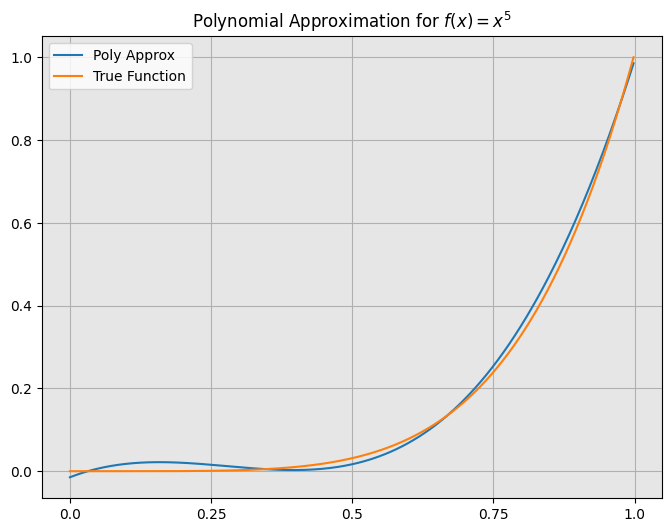
\includegraphics[width=0.35\textwidth]{Figures/FirstRemez15.png}     
    \end{subfigure}%
    \hspace{10mm}
    \begin{subfigure}
        \centering
        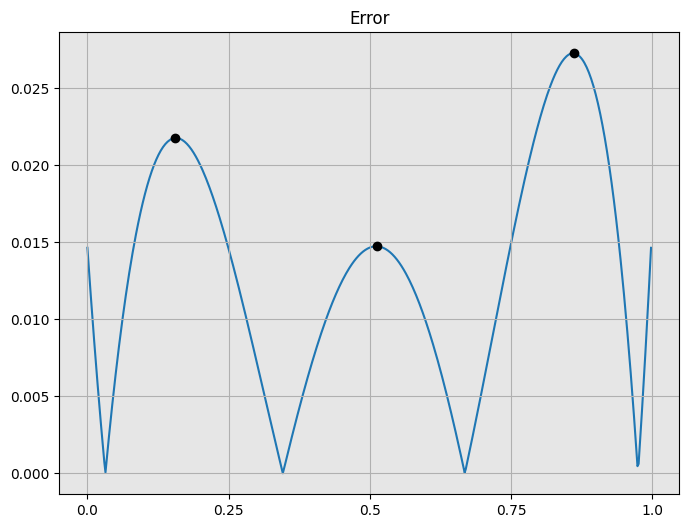
\includegraphics[width=0.35\textwidth]{Figures/Error15.png}    
    \end{subfigure}
    \caption{The first iteration of the Remez Algorithm for $f(x) = x^5$. The coefficients and error are given above. Figure 2: Error for the first iteration. Local maxima are given in black.}
    \label{fig:firstRemez15}
\end{figure}



\newpage
\subsection{Exercise 15, part 2}
Write a code to use the Remez algorithm to compute the best polynomial approximation to $x^5$ by polynomials of degree at most 3 on the interval [0, 1]. Plot the equioscillation points and the error as a function of iteration number. Show plots for initialization both with equispaced points and random initial points.
\partbreak
\begin{solution}

    I have (hopefully) implemented the Remez algorithm correctly, using either a uniform distribution of initial points or a random distribution (uniform distribution, apologies for the overlap in terminology). The uniform distribution is shown in Figure \ref{fig:RemezFinal}, next to the random distribution of points. The random initization did not produce an egregiously bad polynomial, which can happen for initial points being too close to each other.  
\end{solution}

\vspace{1in}
\begin{figure}[!hb]
\centering
    \begin{subfigure}
        \centering
        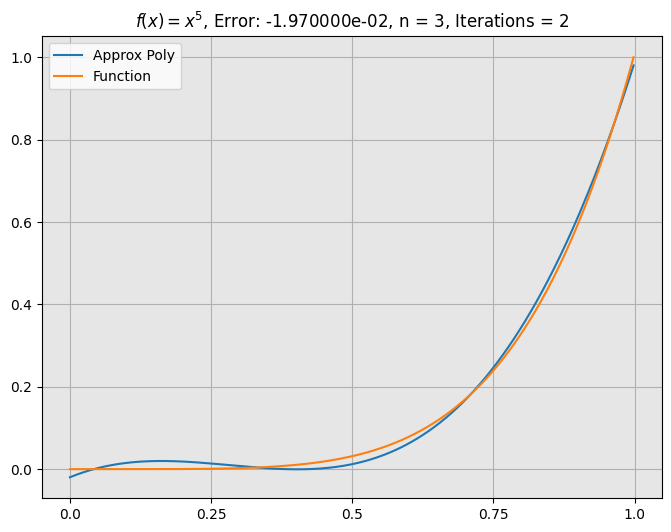
\includegraphics[width = 0.4\textwidth]{Figures/RemezFinalUnif.png}
    \end{subfigure}
    \begin{subfigure}
        \centering
        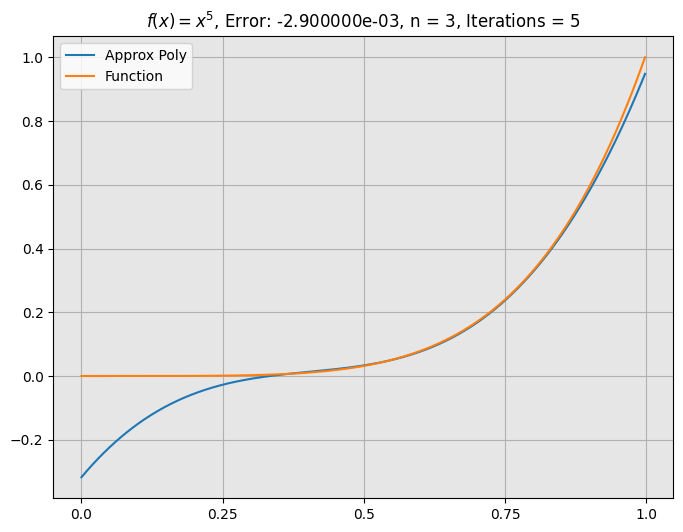
\includegraphics[width = 0.4\textwidth]{Figures/RemezFinalRandom.png}
    \end{subfigure}
    \caption{The Remez algorithm initialized with (left) uniform points and (right) random points. Iterations, degree, and Error are given in each}
    \label{fig:RemezFinal}
\end{figure}

\newpage
\subsection{Exercise 15, part 3}
Extend your code in some way (multiple points at once, more general function, more stable formulae for solving the linear system, some different experiments, etc.).
\partbreak
\begin{solution}

    I have written my code flexible enough to work on any given function (within reason). I have also taken into consideration numerical stability with respect to solving the system of equations. I am solving the system via LU decomposition with partial pivoting, then solving. I have tested my algorithm on the Heavyside function, using a polynomial of degree 30, and investigating the first, second, and 4000-th iteration of the algorithm. The output is given below. Note that I cut off the edges of the domain so we can see the influence of each iteration. 
\end{solution}
\vspace{1in}
\begin{figure}[!hb]
    \centering
    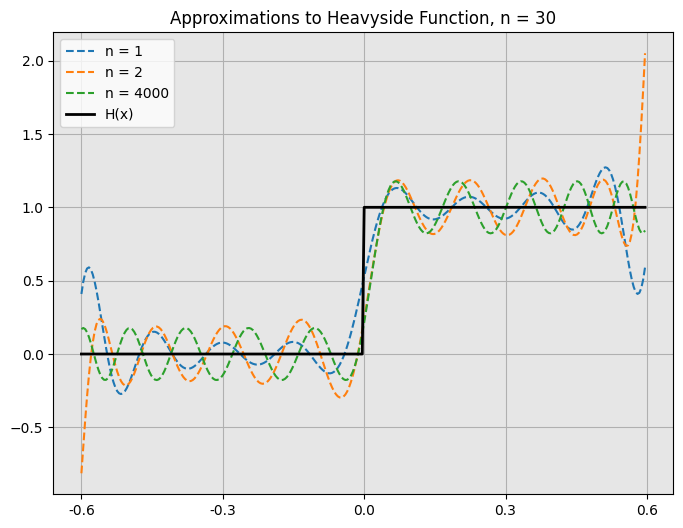
\includegraphics[width = 0.6\textwidth]{Figures/RemezHeavyside.png}
    \caption{Approximations to Heavyside function. The error on the 4000-th iterate is roughly -0.17. The behavior of the error changes drastically for different degree approximations.}
    \label{fig:RemezHeavyside}
\end{figure}
\newpage
\section{Exercise 16}
Recall the formula for Chebyshev polynomials:
\[T_n(x) = \cos(n\arccos(x)).\]
\subsection{Exercise 16, part 1}
Let $p \in P_n$ be a polynomial given by a finite Chebyshev series
\[p(x) = \sum_{k = 0}^n \alpha_k T_k(x)\]
and let $s \in [-1, 1]$. Show that $p(s)$ can be evaluated using the following algorithm. Set $u_{n+1} = 0, u_n = \alpha_n$ and 
\[u_k = 2su_{k+1} - u_{k+2} + \alpha_k, \quad k = n - 1, n - 2, ..., 0.\]
Then $p(s) = \frac{1}{2}(\alpha_0 + u_0 - u_2).$

\newpage
\subsection{Exercise 16, part 2}
Show that $T_n$ satisfies the ODE $(1 - x^2)y'' - xy' + n^2y = 0$.

\newpage
Good optional practice:
Exercise 12???

Fun optional problem:
Exercise 17


\end{document}